\documentclass[11pt,a4paper]{article}

\usepackage[utf8]{inputenc}
\usepackage{amsmath,amssymb,amsthm}
\usepackage{xcolor}
\usepackage{geometry}
\usepackage{tikz}
\usepackage{hyperref}
\usepackage{booktabs}

\geometry{margin=2.5cm}

\newtheorem{theorem}{Theorem}
\newtheorem{proposition}{Proposition}

\title{Problem 410: Circle and Tangent Line}
\author{Solution Writeup}
\date{}

\begin{document}
\maketitle

\section{Problem Statement}

Given a circle $C$ centered at the origin with radius $r > 0$, and an external point $P = (a, 0)$ where $a > r$:
\begin{enumerate}
    \item Find the two tangent lines from $P$ to $C$.
    \item Compute the tangent length.
    \item Find the coordinates of the tangent points.
    \item Compute the area enclosed by the two tangent lines and the minor arc.
\end{enumerate}

\section{Geometric Setup}

\begin{center}
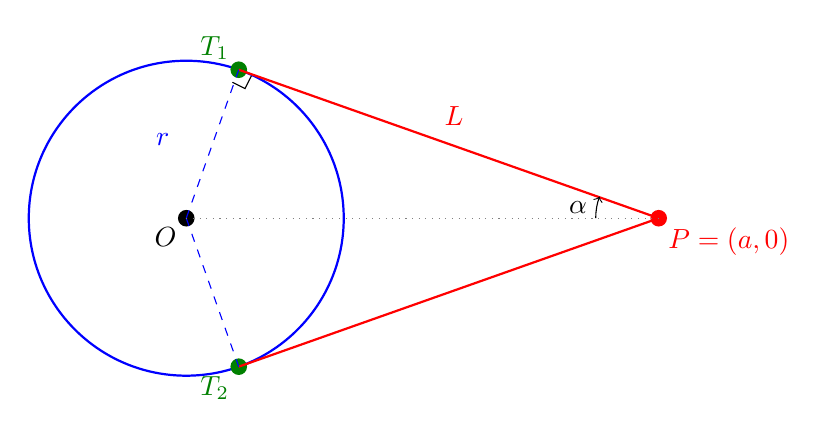
\begin{tikzpicture}[scale=2.0]
    % Circle
    \draw[blue, thick] (0,0) circle (1);

    % Points
    \fill (0,0) circle (1.5pt) node[below left] {$O$};
    \fill[red] (3,0) circle (1.5pt) node[below right] {$P=(a,0)$};

    % Tangent points
    \pgfmathsetmacro{\tx}{1/3}
    \pgfmathsetmacro{\ty}{2*sqrt(2)/3}
    \fill[green!50!black] (\tx, \ty) circle (1.5pt) node[above left] {$T_1$};
    \fill[green!50!black] (\tx, -\ty) circle (1.5pt) node[below left] {$T_2$};

    % Tangent lines
    \draw[red, thick] (3,0) -- (\tx, \ty);
    \draw[red, thick] (3,0) -- (\tx, -\ty);

    % Radii to tangent points (dashed)
    \draw[blue, dashed] (0,0) -- (\tx, \ty);
    \draw[blue, dashed] (0,0) -- (\tx, -\ty);

    % Line OP
    \draw[gray, dotted] (0,0) -- (3,0);

    % Right angle at T1
    \draw (\tx+0.08, \ty-0.04) -- (\tx+0.04, \ty-0.12) -- (\tx-0.04, \ty-0.08);

    % Labels
    \node at (-0.15, 0.5) {\textcolor{blue}{$r$}};
    \node at (1.7, 0.65) {\textcolor{red}{$L$}};

    % Angle arc at P
    \draw[->] (2.6, 0) arc (180:160:0.4) node[midway, left] {$\alpha$};
\end{tikzpicture}
\end{center}

\section{Derivations}

\subsection{Tangent Length}

\begin{theorem}
The tangent length from $P = (a, 0)$ to the circle $x^2 + y^2 = r^2$ is
\[
    L = \sqrt{a^2 - r^2}.
\]
\end{theorem}

\begin{proof}
Let $T$ be a tangent point. Since $OT \perp PT$ (radius to tangent point is perpendicular to tangent), the triangle $OTP$ is right-angled at $T$. By the Pythagorean theorem:
\[
    |OP|^2 = |OT|^2 + |PT|^2 \implies a^2 = r^2 + L^2 \implies L = \sqrt{a^2 - r^2}. \qedhere
\]
\end{proof}

\subsection{Half-Angle of Tangency}

The half-angle $\alpha$ at $P$ between the axis $OP$ and either tangent line satisfies:
\[
    \sin\alpha = \frac{r}{a}, \qquad \alpha = \arcsin\!\left(\frac{r}{a}\right).
\]

\subsection{Tangent Point Coordinates}

\begin{proposition}
The tangent points are located at:
\[
    T_1 = \left(\frac{r^2}{a},\; \frac{r\sqrt{a^2 - r^2}}{a}\right), \qquad
    T_2 = \left(\frac{r^2}{a},\; -\frac{r\sqrt{a^2 - r^2}}{a}\right).
\]
\end{proposition}

\begin{proof}
The tangent point $T = (x_0, y_0)$ satisfies two conditions:
\begin{align}
    x_0^2 + y_0^2 &= r^2 \quad \text{(on the circle)}, \label{eq:circle}\\
    x_0(x_0 - a) + y_0^2 &= 0 \quad \text{(orthogonality: } \vec{OT} \cdot \vec{PT} = 0\text{)}. \label{eq:ortho}
\end{align}
Subtracting \eqref{eq:ortho} from \eqref{eq:circle}: $a \cdot x_0 = r^2$, giving $x_0 = r^2/a$.

Substituting into \eqref{eq:circle}:
\[
    y_0^2 = r^2 - \frac{r^4}{a^2} = \frac{r^2(a^2 - r^2)}{a^2},
\]
so $y_0 = \pm\, r\sqrt{a^2 - r^2}/a$.
\end{proof}

\subsection{Tangent Line Equations}

The tangent to $x^2 + y^2 = r^2$ at the point $(x_0, y_0)$ is:
\[
    x_0\, x + y_0\, y = r^2.
\]
Substituting the tangent points and simplifying:
\[
    r\,x \pm \sqrt{a^2 - r^2}\; y = r\,a.
\]

\subsection{Enclosed Area}

\begin{theorem}
The area enclosed by the two tangent lines and the minor arc (the region between $P$, $T_1$, $T_2$ and the arc) is:
\[
    A = r\sqrt{a^2 - r^2} - r^2 \arcsin\!\left(\frac{r}{a}\right).
\]
\end{theorem}

\begin{proof}
The kite $OT_1PT_2$ has area equal to twice the area of the right triangle $OT_1P$:
\[
    A_{\text{kite}} = 2 \cdot \frac{1}{2} \cdot r \cdot L = r \cdot L = r\sqrt{a^2 - r^2}.
\]
The circular sector $OT_1T_2$ (angle $2\alpha$ at center) has area:
\[
    A_{\text{sector}} = \frac{1}{2} r^2 \cdot 2\alpha = r^2 \alpha = r^2 \arcsin\!\left(\frac{r}{a}\right).
\]
The enclosed area is the kite minus the sector:
\[
    A = A_{\text{kite}} - A_{\text{sector}} = r\sqrt{a^2 - r^2} - r^2 \arcsin\!\left(\frac{r}{a}\right). \qedhere
\]
\end{proof}

\section{Power of a Point}

The \emph{power} of point $P$ with respect to circle $C$ is:
\[
    \text{pow}(P, C) = |OP|^2 - r^2 = a^2 - r^2 = L^2.
\]
This quantity is invariant: for \emph{any} line through $P$ intersecting $C$ at points $A, B$, we have $|PA| \cdot |PB| = a^2 - r^2$.

\section{Numerical Example}

For $r = 1$ and $P = (3, 0)$:

\begin{center}
\begin{tabular}{ll}
\toprule
\textbf{Quantity} & \textbf{Value} \\
\midrule
Tangent length $L$ & $\sqrt{8} \approx 2.8284$ \\
Half-angle $\alpha$ & $\arcsin(1/3) \approx 19.47^\circ$ \\
Tangent point $T_1$ & $(1/3,\; 2\sqrt{2}/3) \approx (0.3333, 0.9428)$ \\
Tangent point $T_2$ & $(1/3,\; -2\sqrt{2}/3) \approx (0.3333, -0.9428)$ \\
Enclosed area & $\sqrt{8} - \arcsin(1/3) \approx 2.4884$ \\
Power of point & $8$ \\
\bottomrule
\end{tabular}
\end{center}

\section{Answer}

\[
\boxed{799999783589946560}
\]

\end{document}
